\section{Teoría de Arnold-Liouville}\label{sec:arnoldliouville}
A la hora de estudiar sistemas dinámicos, una cuestión interesante a plantearse, con consecuencias prácticas y también de carácter fundamental, es si las ecuaciones del sistema podrán ser «integradas», es decir, si podrán ser resueltas mediante integrales definidas («cuadraturas») de funciones conocidas. Decimos entonces que una ecuación diferencial es \emph{integrable por cuadraturas} si es posible escribir su solución general en términos de sumas, productos, composiciones e integrales de funciones conocidas. 

En 1885, Joseph Liouville encontró una condición necesaria para que las ecuaciones de Hamilton de ciertos sistemas hamiltonianos fueran (localmente) integrables por cuadraturas. Décadas más tarde, con la introducción del formalismo geométrico y topológico al estudio de los sistemas dinámicos se descubrirían muchas más cosas interesantes sobre los sistemas que cumplían la condición que Liouville propuso. Destaca especialmente en todo este estudio la teoría de los toros invariantes desarrollada por Vladimir Arnold en 1963. Nace así la teoría de los \emph{sistemas integrables}, cuyos resultados más básicos constituyen el \emph{teorema de Arnold-Liouville}.

\begin{defn}
  \em
  Sea $(M,H)$ un sistema hamiltoniano con $\dim(M)=2n$. Decimos que $(M,H)$ es \emph{integrable (en el sentido de Liouville)} si existen $F_1(=H),\dots,F_n\in \mathcal{C}^{\infty}(M)$ tales que
\begin{enumerate}
  \item son \emph{funcionalmente independientes}, es decir, $\dd F_{1,x}\wedge \dots \wedge \dd F_{n,x}\neq 0$ para casi todo punto\footnote{Aquí con \emph{para casi todo punto} queremos decir que estos puntos forman un conjunto denso.}, 
  \item están \emph{en involución}, esto es, $\pois{F_i}{F_j}=0$ para cada $i,j=1,\dots,n$, y
  \item  los campos $X^{F_i}$ son completos para cada $i=1,\dots,n$. 
\end{enumerate}
Nótese que, como $F_1=H$, en particular, todas las funciones $F_1,\dots,F_n$ son integrales primeras del sistema.

Si escribimos $F:M\rightarrow \RR^n$ con $F(x)=(F_1(x),\dots,F_n(x))$. Los puntos $x\in M$ en los que $\mathrm{rango} (\dd F_x) =n$ se dicen \emph{puntos regulares} del sistema. Los puntos que no son regulares se dicen \emph{puntos críticos}. Si $x\in M$ es un punto crítico, $F(x)$ se dice un \emph{valor crítico}. Si $\Sigma$ es el conjunto de los puntos críticos, $F(\Sigma)\in \RR^n$ se llama \emph{diagrama de bifurcación} del sistema.
 Nótese que, por el teorema de Sard, el diagrama de bifurcación tiene medida nula.
\end{defn}

\begin{thm}[Arnold-Liouville]\label{arnold}
Sea $(M,H)$ un sistema integrable en el sentido de Liouville con $F_1,\dots,F_n$ las funciones en involución.

   Sea $x\in M$ un punto regular del sistema y sea $a=F(x)$. Entonces la componente conexa $M_a$ del conjunto de nivel $F^{-1}(a)$ que contiene a $x$ es una variedad diferenciable invariante bajo el flujo del sistema y $\left. \omega \right|_{M_a}=0$.
  
 Además $M_a$ es difeomorfa a $\TT^k\times \RR^{n-k}$, para cierto $0 \leq k \leq n$. En particular, si $M_a$ es compacta, $M_a$ es difeomorfa al toro $n$-dimensional $\TT^n$. En este caso, se dice que $M_a$ es un \emph{toro invariante}. 
 
 Podemos tomar unas coordenadas $\lambda=(\lambda_1,\dots\lambda_n)$ en $M_a$ de manera que existen unas velocidades constantes $\nu(a)=(\nu_1(a),\dots,\nu_n(a))$ tales que $\dot \lambda (t)=\nu$.

  Existe un entorno $U\subset M$ de cada $M_a$ difeomorfo a $\RR^n \times M_a$ (se dice \emph{entorno tubular}) y un sistema de coordenadas de Darboux $(J,w)=(J_1,\dots,J_n,w_1,\dots,w_n)$ (llamadas \emph{variables de acción-ángulo}\footnote{Las $w_i$ suelen llamarse variables de ángulo ya que, en el caso en que $M_a$ es compacta, son precisamente coordenadas angulares en el toro $M_a$. Las $J_i$ se llaman variables de acción debido a sus dimensiones físicas, en efecto, como las $w_i$ son adimensionales, las $J_i$ tienen que tener dimensiones de Posición$\times$Momento Lineal, que son precisamente las dimensiones de la integral de acción (citar caso lagrangiano).}) en $U$ tales que las $w_i$ son coordenadas en $M_a$ y las $J_i$ son constantes en cada $M_a$. Como consecuencia, las ecuaciones de Hamilton del sistema son integrables por cuadraturas.
\end{thm}

Cabe hacer un breve comentario sobre la historia de este resultado.
Como ya se ha comentado, la formulación original, en términos de mecánica hamiltoniana clásica, se debe a Liouville en 1855, mientras que la teoría moderna la desarrolló Arnold en 1963. Por otra parte, las variables de acción-ángulo fueron introducidas originalmente por Delaunay en 1860 para estudiar el movimiento de la Luna y más tarde, a principios del siglo XX, usadas por los físicos para estudiar el átomo de Bohr, siendo Schwarzschild el que acuñara esa terminología en 1916. La obtención formal de las variables de acción-ángulo se atribuye a Mineur en 1936. 
 Una discusión más extensa sobre la historia del teorema de Arnold-Liouville puede encontrarse en las páginas 640 y 641 del texto de Spivak \cite{spivak}.

 Podemos dar entonces la demostración, que haremos en varios pasos.

 \begin{proof}
  En primer lugar, como $x$ es regular, $F$ tiene rango máximo en cada punto de $M_a$ y, por el teorema de la función implícita, $M_a$ es una subvariedad regular de $M$ de dimensión $2n-n=n$. 
  Como $M$ es una variedad simpléctica, para cada $i=1,\dots,n$, podemos definir el campo $X_i=X^{F_i}$. Al ser las $\dd F_i$ linealmente independientes los campos $X_i$ son linealmente independientes. Además, por el teorema de Noether, como para cada $i,j= 1,\dots,n$ $\pois{F_i}{F_j}=0$ (luego es constante), entonces $\lie{X_i}{X_j}=0$. Por esto mismo, la derivada de la función $F_i$ en la dirección de $X_j$ es 0, luego los campos $X_j$ son tangentes a $M_a$.

  De aquí sacamos varias conclusiones:
  \begin{enumerate}
    \item $M_a$ es invariante con respecto a cada uno de los $n$ flujos hamiltonianos generados por cada función $F_i$ (luego, en particular lo será respecto del generado por $F_1$).
    \item Como, para cada $x \in M_a$, los campos $X_1|_x,\dots, X_n|_x$ forman una base de $T_x M_a$, sean $X_x, Y_x \in T_x M_a$, entonces $X_x = \sum_{i=1}^n b_i X_i|_x$, $Y_x=\sum_{i=1}^n c_i X_i|_x$. Ahora,
      \[
	\omega(X_x,Y_x)= \sum_{i,j=1}^n b_i c_j \omega(X_i|_x,X_j|_x) = \sum_{i,j=1}^n b_i c_j \{F_j,F_i\} = 0.
      \]
      Por tanto, $\omega$ se anula en $T_x M_a$. 
    \item $M_a$ es una variedad diferenciable de dimensión $n$ con $n$ campos conmutativos dos a dos y linealmente independientes en todo punto de $M_a$. 
  \end{enumerate}

  Esto prueba la primera parte del teorema. Para continuar, necesitamos probar un lema previo.

  \begin{lema}\label{lemtoro}
    Sea $M$ una variedad diferenciable de dimensión $n$ conexa y compacta tal que existen campos $X_1,\dots,X_n$ en $M$ completos y linealmente independientes y tales que, para todo $i,j=1,\dots,n$, $i\neq j$, $[X_i,X_j]=0$. Entonces $M$ es difeomorfa al $\TT^k\times \RR^{n-k}$. 
\end{lema}
\begin{proof}(del Lema \ref{lemtoro}).
  Para cada $i=1,\dots,n$, sea $g_i$ el flujo completo generado por $X_i$. Como para todo $i\neq j$ $[X_i,X_j]=0 $ entonces $g_i$ conmuta con $g_j$, es decir, $g_ig_j (x)=g_jg_i (x)$, para todo $x \in M$. 

  Así, podemos definir una acción de $\RR^n$ en $M$ que a cada $t=(t_1,\dots,t_n)\in \RR^n$ le asigna $g_t:M\rightarrow M,$ con $g_t=g_{1,t_1}\cdots g_{n,t_n}$.
Por conmutar los flujos, $g_{t+s}=g_t g_s$. Ahora, fijo $x_0 \in M$, definimos 
\[
  \begin{array}{rcl}
g:\RR^n & \longrightarrow & M \\
t & \longmapsto & g_t (x_0).
\end{array}
\]

Como los campos son linealmente independientes, $d_t g$ es un isomorfismo lineal para todo $t$ y, por el teorema de la función implícita, $g$ es un difeomorfismo local. Además, sea $x\in M$, tomamos una curva $\gamma$ que una $x$ y $x_0$ y una sucesión finita de entornos $V_1,\dots,V_n$ que recubran $\gamma$, en los que $g$ sea difeomorfismo y tales que $x_0 \in V_1$, $x \in V_n$. Para cada $i=1,\dots,n-1$, sea $x_i \in V_i \cap V_{i+1}$ y sea $x_n=x$. Para cada $i=0,\dots,n-1$, centramos $g$ en $x_i$ (de tal forma que $g(0)=x_i$) en el entorno $V_{i+1}$ y lo llamamos $g_i$. Definimos $t_i$ tal que $g_{i-1,t_i}(x_{i-1})=x_i$, entonces,
\[
  x=g_{n-1,t_n}(x_{n-1})=g_{n-1,t_n}g_{n-2,t_{n-1}}(x_{n-2})=\cdots=g_{n-1,t_{n}}\cdots g_{0,t_1} (x_0),
\]
luego, sea $t=t_1+\cdots+t_n$, $x=g_t (x_0)$. Por tanto, $g$ es sobreyectiva.
\begin{figure}[h]
  \centering
  \includegraphics[width=0.5\textwidth]{pics/entornos.eps}
  \caption{Idea de la demostración de que $g$ es sobreyectiva.}
  \label{fig:entornos}
\end{figure}

Tenemos entonces que $g:\RR^n\rightarrow M$ es un difeomorfismo local sobreyectivo, luego es una identificación diferenciable, de modo que si llamamos 
\[  
  H:=\{t \in \RR^n \mid g_t(x_0)=x_0\},
\]
entonces, por la propiedad universal del cociente, el siguiente diagrama
\begin{center}
  \begin{tikzcd}
    \RR^n \arrow{r}{g}\arrow{d}{} & M    \\ 
    \RR^n/H, \arrow{ru}{}
  \end{tikzcd}
\end{center}
da un difeomorfismo entre $M$ y $\RR^n/H$. Si $H$ es vacío, $M\cong \RR^n$ y habríamos terminado. Supongamos que $H$ es no vacío.
 Entonces, dados $t, s \in H$, 
\[
  g_{s+t}(x_0)=g_sg_t(x_0)=g_s(x_0)=x_0
\]
y 
\[
  g_{-t}(x_0)=g_{-t}g_t(x_0)=x_0.
\] 
Es decir, $H$ es un subgrupo de $(\RR^n,+)$. Además, $H$ no depende de la elección de $x_0$, en efecto, si $x=g_r (x_0)$ y $t\in H$, entonces 
\[
  g_t (x) = g_{t+r}(x_0)=g_rg_t(x_0)=g_r(x_0)=x. 
 \] 

 Como $g$ es un difeomorfismo local, existe un entorno $V\subset \RR^n$ de 0 tal que $H\cap V= \{0\}$. Es más, sean $t\in H$, $s\in V\backslash \{0\}$ y $x\in M$, 
  \[
    g_{t+s}(x)=g_sg_t(x)=g_s(x)\neq x.
  \]
  Luego $H$ es un conjunto discreto. 
  \begin{figure}[h]
    \centering
    \includegraphics[width=0.2\textwidth]{pics/discreto}
    \caption{Idea de que $H$ es discreto.}
    \label{fig:discreto}
  \end{figure}

  Antes de continuar, es necesario probar el siguiente lema:

  \begin{lema}\label{discreto}
    Todo subgrupo no trivial, cerrado y discreto $H$ de $\RR^n$ es isomorfo a $\ZZ^k$ para algún $k\in\{1,\dots,n\}$. Es decir, existen $e_1,\dots,e_k \in H$ linealmente independientes tales que 
    \[
      H=\{n_1e_1+\cdots+n_ke_k \mid (n_1,\dots,n_k) \in \ZZ^k \}.
    \]
  \end{lema}
  \begin{proof}(del Lema \ref{discreto}). 
  Sea $e_0 \in H$, $e_0 \neq 0$. Como $H$ es discreto, $H \cap B(0,\norm{e_0})$ es finito. De estos puntos, consideramos aquellos que están en $L(e_0)$ \footnote{Aquí $L(x)$ denota la envoltura lineal de $x$.} y de estos escogemos el más cercano, que llamaremos $e_1$. 
  
  Si existieran algún $e \in H$ y algún $m \in \ZZ$ tal que $e \in (me_1,(m+1)e_1)$, entonces $e-me_1 \in H \cap L(e_0)$ estaría más cerca de 0 que $e_1$. Por tanto, 
  \[
    H\cap L(e_0) = e_1\ZZ.
  \]

  Si no hay puntos de $H$ fuera de $L(e_1)$ hemos terminado, $H$ es isomorfo a $\ZZ$. En caso contrario, sea $e \in H \backslash L(e_1)$, proyectamos ortogonalmente $e$ sobre $L(e_1)$. Esta proyección cae exactamente sobre un intervalo $\Delta=[me_1,(m+1)e_1)$ para cierto $m \in \ZZ$. Sea $C$ el cilindro de eje $\Delta$ y de radio igual a la distancia entre $\Delta$ y $e$. $C\cap H$ es finito. De estos puntos, sea $e_2$ el más cercano a $\Delta$ que no esté en $\Delta$. Entonces, para cualquier otro $f \in H$, la distancia entre $f$ y $L(e_1)$ es mayor que la distancia entre $e_2$ y $L(e_1)$. 
    
    En efecto, en tal caso, sea $l \in \ZZ$ tal que la proyección ortogonal de $f$ cae sobre $[le_1,(l+1)e_1)$, entonces $f'=f-le_1+me_1 \in C$ y la distancia entre $f'$ y $L(e_1)$ es menor que la distancia entre $e_2$ y $L(e_1)$, lo que nos lleva a una contradicción.

  \begin{figure}[h]
    \centering
    \includegraphics{pics/grupo}
    \caption{Idea de la demostración del lema.}
    \label{fig:grupo}
  \end{figure}

      Ahora, $\{n_1e_1+n_2e_2 \mid (n_1,n_2) \in \ZZ^2 \}$ forma una red discreta en $L(e_1,e_2)$. Además, si existiera un $e\in H$ que no perteneciese a la red, sean $m_1=[\esc{e}{e_1}]$, $m_2=[\esc{e}{e_2}]$. Entonces, $e-m_1e_1-m_2e_2$ estaría más cerca de $L(e_1)$ que $e_2$. Por tanto, esta red es exactamente $L(e_1,e_2) \cap H$.

      Procedemos ahora por inducción, supongamos que existen $e_1,\dots,e_k$ linealmente independientes tales que $\{n_1e_1+\cdots+n_ke_k \mid (n_1,\dots,n_k) \in \ZZ^k \} = L(e_1,\dots,e_k) \cap H$ y que existe $e\in H$ tal que $e \not\in L(e_1,\dots,e_k)$. Análogamente, la proyección ortogonal de $e$ sobre $L(e_1,\dots,e_k)$ cae sobre un hipercubo $\Delta=[m_1e_1,(m_1+1)e_1) \times \cdots \times [m_ke_k,(m_k+1)e_k)$. Sea $C$ el conjunto de los puntos cuyas proyecciones ortogonales caen en $\Delta$ y más cercanos a $\Delta$ que $e$, entonces $C \cap H$ es finito. Sea $e_{k+1}$ el más cercano a $\Delta$ de estos puntos, que no esté en $\Delta$. Para cualquier otro $f \in H$, la distancia entre $f$ y $L(e_1,\dots,e_k)$ es mayor que entre $e_2$ y $L(e_1,\dots,e_k)$, por un razonamiento completamente análogo al caso bidimensional. 

	Por tanto, $\{n_1e_1+\dots+n_{k+1}e_{k+1} \mid \in \ZZ^{k+1}\}$ forma una red discreta en $L(e_1,\dots,e_{k+1})$ y, de forma análoga al caso anterior, esta red agota los puntos de $H\cap L(e_1,\dots,e_{k+1})$.

	Finalmente, sea $k$ el mínimo número natural tal que no existe $e \in H \backslash L(e_1,\dots,e_k)$. Entonces $H$ es isomorfo a $\ZZ^k$.
\end{proof}

Terminamos ahora la demostración del Lema \ref{lemtoro}.
 
  Sea $k$ el número de generadores de $H$ y sea la proyección natural
  \[
    \begin{array}{rcl}
      \varpi: \RR^n = \RR^k \times \RR^{n-k} & \longrightarrow & \TT^k \times \RR^{n-k} \\
      (x,y) & \longmapsto & (\exp(x), y).
    \end{array}
  \]
  En particular, $\varpi$ da un homomorfismo de grupos cuyo núcleo es un subgrupo discreto de $\RR^n$ generado por $u_1,\dots,u_k \in \RR^n$. 
  Sean $e_1,\dots,e_k$ los generadores de $H$ y sea $B:\RR^n \rightarrow \RR^n$ un isomorfismo lineal tal que cada $u_i$ va a parar a $e_i$. Entonces, la aplicación $\tilde{B}$ que hace el siguiente diagrama conmutativo es un difeomorfismo,
  \begin{center}
    \begin{tikzcd}
  \RR^n    \arrow{r}{B}\arrow{dd}[anchor=east]{\varpi} & \RR^n\arrow{dd}[anchor=west]{g} \\ 
  & \\
  \TT^k \times \RR^{n-k}\arrow{r}[anchor=south]{\tilde{B}} & \RR^n/H \cong M.
     \end{tikzcd}
   \end{center}
  
\end{proof}

Aplicando directamente el Lema \ref{lemtoro} a $M_a$ tenemos que es difeomorfa a $\TT^k\times \RR^{n-k}$ para cierto $k=0,\dots,n$. En particular, si $M_a$ es compacta, entonces $k=n$ y $M_a\cong \TT^n$. Hemos probado entonces la segunda parte del teorema.

Si consideramos ahora el isomorfismo lineal $B$ (que depende del punto $a$) dado por el diagrama anterior y llamamos $\nu(a)$ a la primera columna de la matriz asociada a $B$, entonces $B(t,0,\dots,0)=\nu(a)t$. Podemos dar entonces unas coordenadas $\lambda:M\rightarrow \RR^n$, donde $\lambda$ es una sección de $\varpi$, es decir, hace el siguiente diagrama conmutativo
\begin{center}
  \begin{tikzcd}
    \RR^k\times \RR^{n-k} \arrow{rd}[anchor=north,rotate=-30]{\varpi} \arrow{r}{\mathrm{id}} & \RR^n    \\ 
    & M. \arrow{u}{\lambda}
  \end{tikzcd}
\end{center}

Ahora, como el flujo del sistema $\varphi^H$ es igual a $g_1$, el siguiente diagrama conmuta
\begin{center}
  \begin{tikzcd}
    \RR^n    & \RR \arrow{l}[anchor=south]{\nu(a) \bullet} \arrow{d}[anchor=west]{\varphi_{\bullet}^H(x)} \\ 
    &M. \arrow{ul}[rotate=-30]{\lambda} 
   \end{tikzcd}
 \end{center}
 Por tanto, $\lambda(t)=\lambda(\varphi_t(x))=\nu(a) t$, luego $\dot \lambda(t)=\nu(a)$. Esto prueba la tercera parte del teorema.

 Para probar la última parte del teorema veamos primero que existe un $U \subset M$ entorno de $M_a$ difeomorfo a $\RR^n \times M_a$. 
 Como $F$ tiene rango máximo, si tomamos $D\cong\RR^{2n}$ entorno simplemente conexo de $x$, existe $V\subset D$ y existe $B\subset \RR^n$ abierto tal que $F|_V:V \rightarrow B$ es un difeomorfismo. Ahora, reduciendo el entorno $V$ si es preciso, sea
  \[
    \begin{array}{rcl}
      \Phi:V & \longrightarrow & \RR^n \times M_a \\
           x & \longmapsto & (F(x), \lambda),
    \end{array}
  \]
  con $\lambda$ las coordenadas antes obtenidas en la componente $M_{F(x)}$ que contiene a $x$. Entonces claramente $\Phi$ da un difeomorfismo entre $U=\bigcup_{x\in V}M_{F(x)}$ (que es un entorno de $M_a$) y $\RR^n \times M_a$.
\begin{obs}
  \em
  Aquí estamos suponiendo que $x$ no está en el borde de $M$, en tal caso procederíamos análogamente para obtener un entorno difeomorfo a $\HH^n \times \TT^n$.
\end{obs}
 \end{proof}

En primer lugar, vamos a considerar un ejemplo característico que aclara alguna de las ideas detrás de esta teoría.
\begin{ejemplo}
  \em
  Consideramos el oscilador armónico unidimensional, con hamiltoniano
  \begin{equation*}
    H(q,p)=\frac{p^2}{2m}+\frac{1}{2}kq^2.
  \end{equation*}
  Por simplicidad, supondremos que la masa y la constante del muelle valen 1, de forma que $H(q,p)=\frac{1}{2}(p^2+q^2)$. Las curvas $C_E$ de energía constante en el espacio de fases $\RR^2$ son circunferencias de centro 0 y radio $a=\sqrt{2E}$, con
  \begin{equation*}
    E=\frac{1}{2}(p^2+q^2).
  \end{equation*}
  \begin{figure}[h]
    \centering
    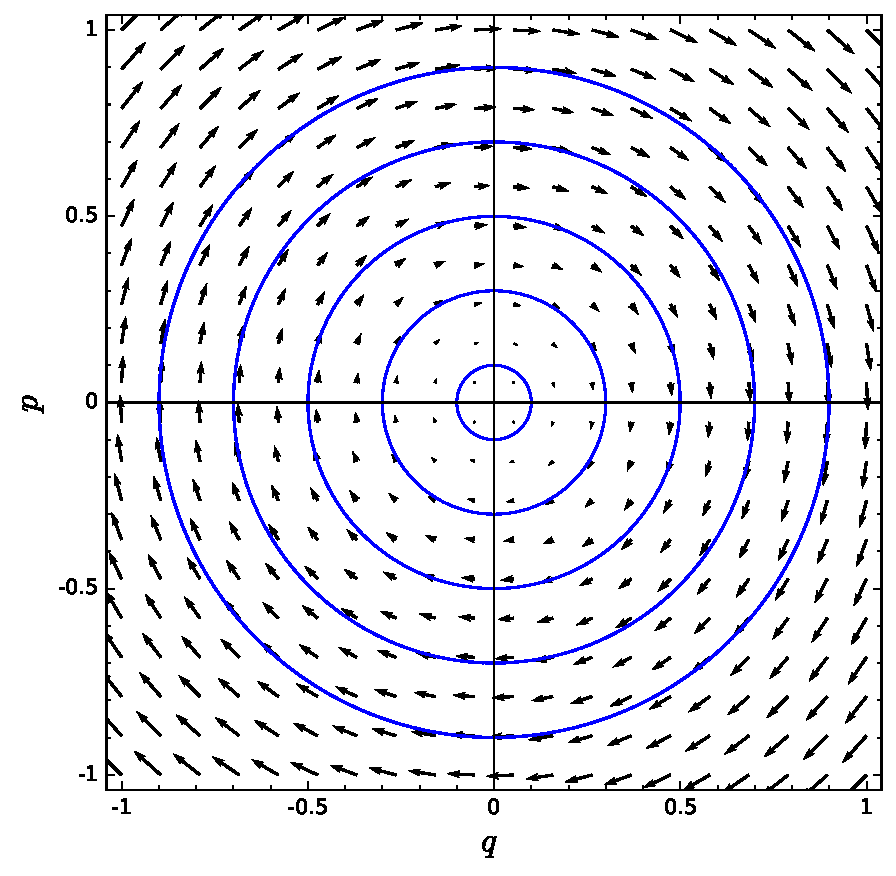
\includegraphics[width=0.4\textwidth]{pics/oscilador}
    \label{fig:oscilador}
    \caption{Espacio de fases del oscilador armónico junto al campo y al flujo hamiltonianos}
  \end{figure}
  Ahora, si tomamos unas coordenadas «polares» $(E,\phi)$, donde $\phi$ es la coordenada angular en cada una de estas circunferencias, la dinámica del sistema queda mucho más simplificada: 
  \begin{align*}
    E(t)&=E(0) \\
    \phi(t)&=\phi(0)+\omega(E(0))t.
  \end{align*}
  Sin embargo, ¿será canónica la transformación $(q,p) \rightarrow (E,\phi)$?
  \begin{figure}[h]
    \centering
    \includegraphics[width=0.6\textwidth]{pics/polar}
    \caption{Cambio de coordenadas $(q,p) \rightarrow (E,\phi)$}
    \label{fig:polar}
  \end{figure}
  En este caso es claro que la transformación preserva el área $\frac{1}{2}a^2\phi$. Más generalmente, si $A$ es una región del plano, 
  \begin{equation*}
    \text{área}(A)= \int_A r \dd r \wedge \dd \phi = \int_A \dd\left(\frac{1}{2}r^2\right) \wedge \dd \phi.
  \end{equation*}
  Por tanto, la transformación es canónica porque precisamente, si $A_E$ es la región encerrada por $C_E$, entonces
  \begin{equation*}
    E=\frac{1}{2}a^2=\frac{1}{2\pi}\text{área}(A_E).
  \end{equation*}

  En las coordenadas originales, esta área es
  \begin{equation*}
    J=\int_{A_E} \dd p \wedge \dd q = \int_{A_E}d (p\dd q) = \int_{C_E} p \dd q,
  \end{equation*}
  donde en el último paso hemos utilizado el teorema de Stokes. Esta $J$ normalmente se conoce como \emph{variable de acción}, debido a sus dimensiones.

  En un caso más general, podemos considerar el sistema formado por $n$ osciladores armónicos acoplados o, equivalentemente, un oscilador armónico $n$-dimensional. El hamiltoniano del sistema será (tomando $k=m=1$)
  \begin{equation*}
    H(q_1,\dots,q_n,p_1,\dots,p_n)= H_1(q_1,p_1)+ \cdots +H_n(q_n,p_n) = \frac{1}{2}(p_1^2+\cdots+p_n^2+q_1^2+\cdots+q_n^2).
  \end{equation*}
  Este sistema es integrable en el sentido de Liouville. Basta tomar $F=(H,H_2+\cdots+H_{n},H_3+\cdots+H_{n-2},\dots,H_n)$, ya que 
  \begin{equation*}
    \pois{H_i}{H_j} = \sum_{k=1}^n \parcial{H_i}{p_k}\parcial{H_j}{q_k} - \parcial{H_j}{p_k}\parcial{H_i}{q_k}= p_iq_j \delta_{ij} - p_jq_i \delta{ij} = p_iq_i-p_iq_i = 0,
  \end{equation*}
  y $\det(F_{*,x}) \neq 0$ para todo $x \in \RR^{2n}$. 
  
  $F^{-1}(a)$ vendrá dado por 
  \begin{equation*}
    \left\lbrace
    \begin{array}{l}
      \frac{1}{2}(p_1^2+q_1^2)=a_1-a_2 \\
      \frac{1}{2}(p_2^2+q_2^2)=a_2-a_3 \\
\vdots \\
\frac{1}{2}(p_n^2+q_n^2)=a_n, 
    \end{array}
    \right.
  \end{equation*}
  que son las ecuaciones de un toro $n$-dimensional.

  Entonces, sean $\gamma_1,\dots,\gamma_n$ una base de ciclos del toro \nota{Esto es muy intuitivo pero hay que escribirlo bien, en los libros pone que son los generadores del grupo de homología de $\TT^n$, cuando dé TOAL a lo mejor sé lo que es}, podemos definir las variables de acción 
  \begin{equation*}
    J_i = \frac{1}{2\pi}\int_{\gamma_i} \sum_{k=1}^n p_k \dd q_k = \frac{1}{2\pi} \int_{\gamma_i} \alpha.
  \end{equation*}
  La definición de estas variables no depende de la base elegida ya que, por el teorema de Stokes,
  \begin{equation*}
    \int_{\gamma_i} \alpha - \int_{\gamma_i'} \alpha = \int_{\sigma} \omega=0,
  \end{equation*}
  donde $\sigma$ es la región encerrada por las curvas y $\omega=0$ en el toro (el cálculo de esto está hecho con precisión más adelante).

Sean las variables angulares $\phi_i$ a lo largo de cada ciclo generado por $\gamma_i$, si $(q,p) \rightarrow (J,\phi)$ es canónica, podemos tomar las variables $(J,\phi)$ en las que la dinámica toma una forma especialmente simple. Esto se debe a que $J=J(a)$, de modo que, por las ecuaciones de Hamilton, 
\begin{equation*}
  \parcial{H}{\phi_i}=-\dot{J_i}=0.
\end{equation*}
Por tanto, $H=H(J_1(a),\dots,J_n(a))$ y 
\begin{equation*}
  \dot{\phi_i}=\parcial{H}{J_i} = \omega_j(a),
\end{equation*}
con $\omega_j$ constante en $M_a$. Las ecuaciones de Hamilton quedan entonces integradas en la forma
\begin{align*}
  J(t)= & J(a) \\
  \phi(t) = & \phi(0) + \omega(a) t.
\end{align*}

No hemos demostrado que el cambio de coordenadas sea un simplectomorfismo, lo que puede hacerse usando el método de Hamilton-Jacobi, que aquí no vamos a exponer. Sin embargo, no nos hará falta, ya que nosotros daremos otra prueba, demostrando un teorema general para construir variables de acción-ángulo en variedades simplécticas.
\end{ejemplo}

Vamos a estudiar también algunos ejemplos de sistemas con funciones en involución, que en ciertos supuestos serán integrables en el sentido de Liouville.
  
\begin{ejemplo}[Péndulo simple]
  \em
  Consideramos un péndulo cuya «cuerda» es una barra rígida de masa despreciable y longitud 1. El espacio de fases del péndulo es el fibrado cotangente de $\SF^1$, que no es otra cosa que un cilindro. Tomando como coordenada generalizada el ángulo $\phi$ de desviación del péndulo respecto de la vertical, el hamiltoniano viene dado por 
  \begin{equation*}
    H(\phi,p)=\frac{1}{2}p^2 - g\cos\phi,
  \end{equation*}
  donde $g$ es la aceleración de la gravedad y hemos tomado el centro como origen de energía potencial.
  \begin{figure}[h]
    \centering
    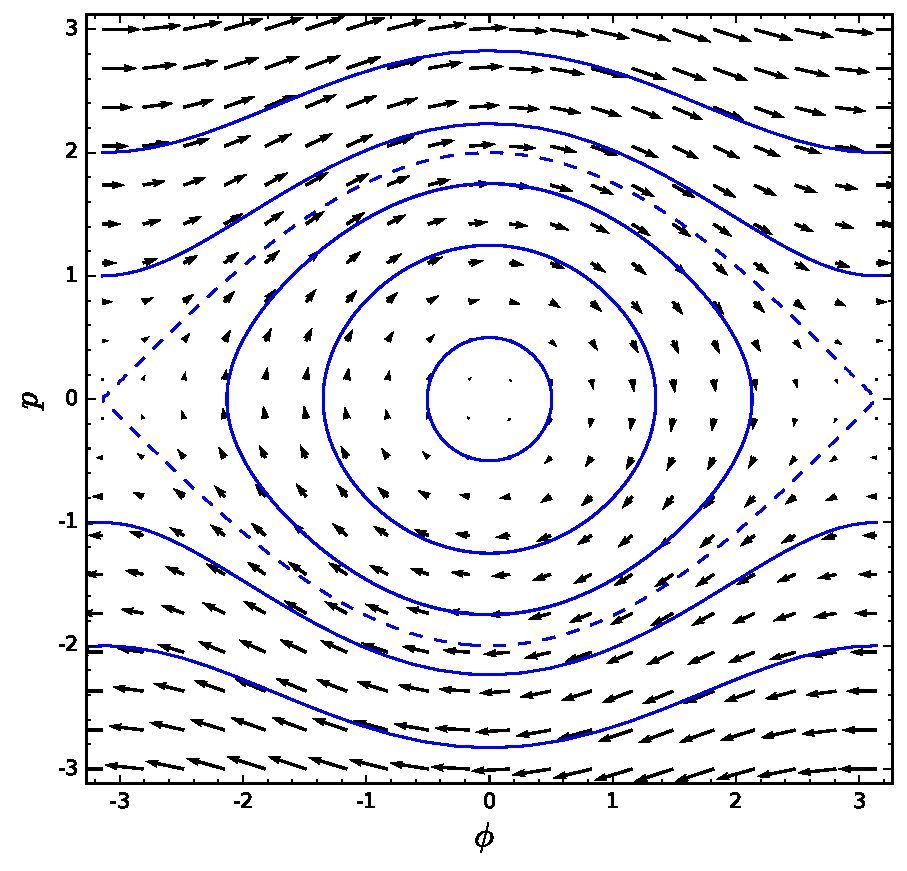
\includegraphics[width=0.4\textwidth]{pics/pendulo}
    \label{fig:pendulo}
    \caption{Espacio de fases del péndulo junto al campo y al flujo hamiltonianos.}
  \end{figure}
  Como podemos ver en la figura \ref{fig:pendulo}  las trayectorias son cerradas, luego cada curva de energía constante es compacta. $\dd H$ será distinta de 0 en todo punto exceptuando los casos $(\phi=0,p=0)$ y $(\phi=\pi,p=0)$, que corresponden a puntos de equilibrio (el primero, estable, el segundo, inestable) donde la trayectoria es sólo un punto. La curva que aparece punteada en la figura \ref{fig:pendulo}, de ecuación
  \begin{equation*}
    g=H(\phi,p)=\frac{1}{2}p^2 - g \cos\phi ,
  \end{equation*}
  corresponde al punto de equilibrio y a dos trayectorias que tienden asintóticamente al punto de equilibrio inestable. Estas trayectorias son matemáticamente factibles aunque su realización práctica parezca una tarea imposible y en ellas no aplica la teoría de Arnold-Liouville, puesto que la curva punteada no es una variedad, al contener un punto con $\dd H=0$. Estas trayectorias se conocen como \emph{singularidades} del sistema. Las curvas que quedan dentro de la curva punteada corresponden a movimientos de oscilación en torno al punto de equilibrio estable, mientras que las que quedan fuera corresponden a movimientos de rotación del péndulo alrededor de su centro. 
\end{ejemplo}
\begin{ejemplo}[Potencial central]
  \em
  Consideramos una partícula que se mueve en $\RR^3$ sometida a un potencial central, esto es, una función $V$ que sólo depende de $r=||x||$. El espacio de fases es $\RR^6$ y el hamiltoniano (tomando $m=1$) viene dado por
  \begin{equation*}
    H(x,p)=\frac{p^2}{2}+V(r).   
  \end{equation*}
  Sea ahora el momento angular
  \begin{equation*}
    L=x \times p,
  \end{equation*}
  cada una de sus componentes es $L_i=\epsilon_{ijk}(x_jp_k-x_kp_j)$, donde $\epsilon_{ijk}$ es la paridad de $(i,j,k)$ como permutación de $(1,2,3)$. Podemos calcular ahora 
  \begin{equation*}
    \pois{H}{L_i}= \sum_{k=1}^3 \parcial{H}{p_k} \parcial{L_i}{x_k} - \parcial{H}{x_k} \parcial{L_i}{p_k}= -\sum_{k=1}^3 \epsilon_{ijk}\left( p_kp_j + \frac{x_kx_j}{r}V'(r) \right)=0.
  \end{equation*}
  Por tanto, $L$ es una cantidad conservada. Al ser $L$ un vector, realmente son cantidades conservadas su norma y su dirección y sentido, lo que implica que se conservan $L^2=\esc{L}{L}$ y $L_3$. Además $\pois{L^2}{L_3}=0$, lo que nos da tres funciones en involución en el sistema.
  Sin embargo, la integrabilidad en sentido de Liouville no está garantizada por los resultados que hemos probado, ya que en general las órbitas pueden ser no acotadas y las funciones no ser independientes. 
\end{ejemplo}
\begin{ejemplo}[Trompo simétrico]
  \em
  Consideremos un trompo simétrico (la clásica peonza de juguete) que gira con su punta fija en un punto. Su espacio de configuración viene dado por las posibles rotaciones de sus ejes principales de inercia ($X',Y',Z'$) respecto a los tres ejes del sistema de laboratorio (la vertical y dos ejes arbitrarios en el suelo, $X,Y,Z$). De modo que el espacio de fases del trompo simétrico es $T^*\mathrm{SO}(3)$. Sean $I_1,I_2,I_3$ los momentos de inercia del trompo, que el trompo sea \emph{simétrico} quiere decir que $I_1=I_2$ y que el centro de masas cae sobre el eje $Z'$. En este caso, tras unos cálculos se obtiene que el hamiltoniano del sistema es
  \begin{equation*}
    H(\theta,\phi,\psi,p_{\theta},p_{\phi},p_{\psi})=\frac{p_{\theta}^2}{2I_1}+\frac{(p_{\phi}-p_{\psi}\cos\theta)^2}{2I_1\sin^2\theta}+\frac{p_{\psi}^2}{2I_3}+Mgl\cos \theta,
  \end{equation*}
  donde $g$ es la aceleración de la gravedad, $M$ es la masa de la peonza, $l$ es la distancia de la punta al centro de masas, $(\theta,\phi,\psi)$ son los ángulos de Euler de la rotación de los ejes principales de inercia respecto a los del laboratorio y $(p_{\theta},p_{\phi},p_{\psi})$ son sus momentos canónicos conjugados. 
  Las frecuencias de giro de cada uno de los ángulos de Euler $\theta$, $\phi$ y $\psi$ se llaman frecuencias de \emph{nutación}, \emph{precesión} y \emph{rotación}, respectivamente.
  \begin{figure}[h]
    \label{fig:euler}
    \centering
    \begin{minipage}[b]{0.4\textwidth}
    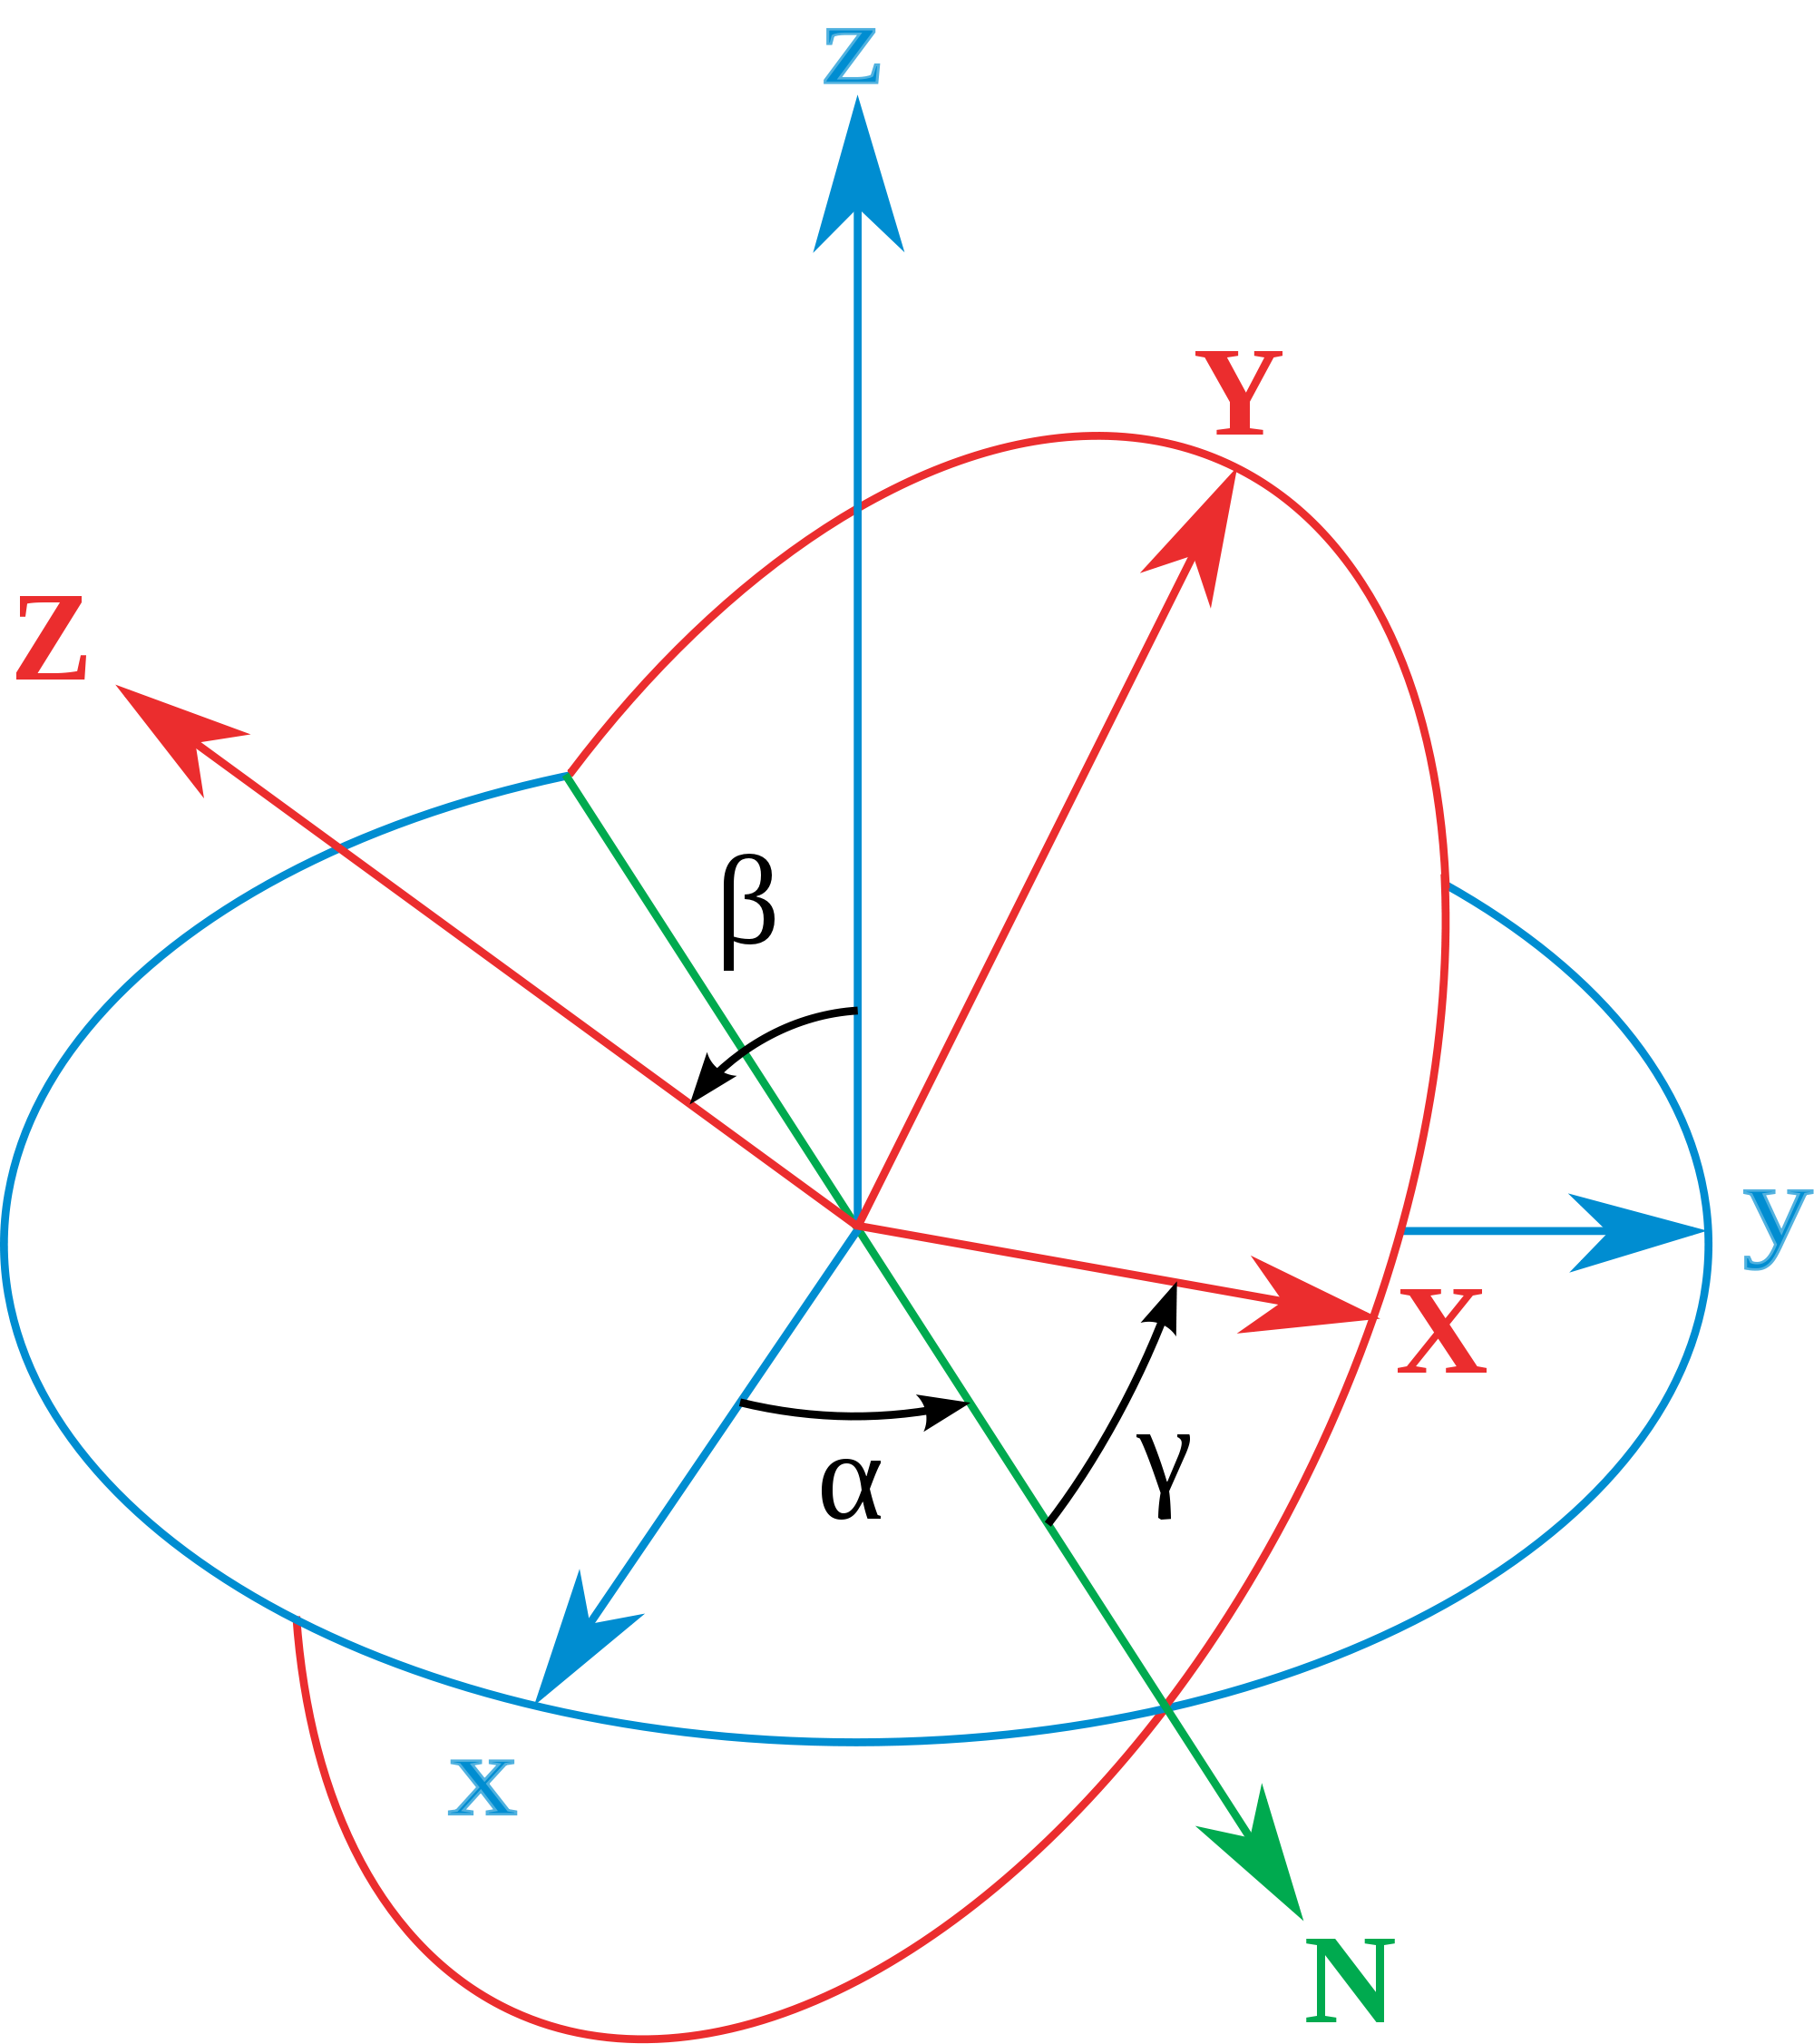
\includegraphics[width=\textwidth]{pics/euler}
    \caption{Construcción de los ángulos de Euler. Fuente: \cite{euler}.}
  \end{minipage}
  \hfill
  \begin{minipage}[b]{0.4\textwidth}
    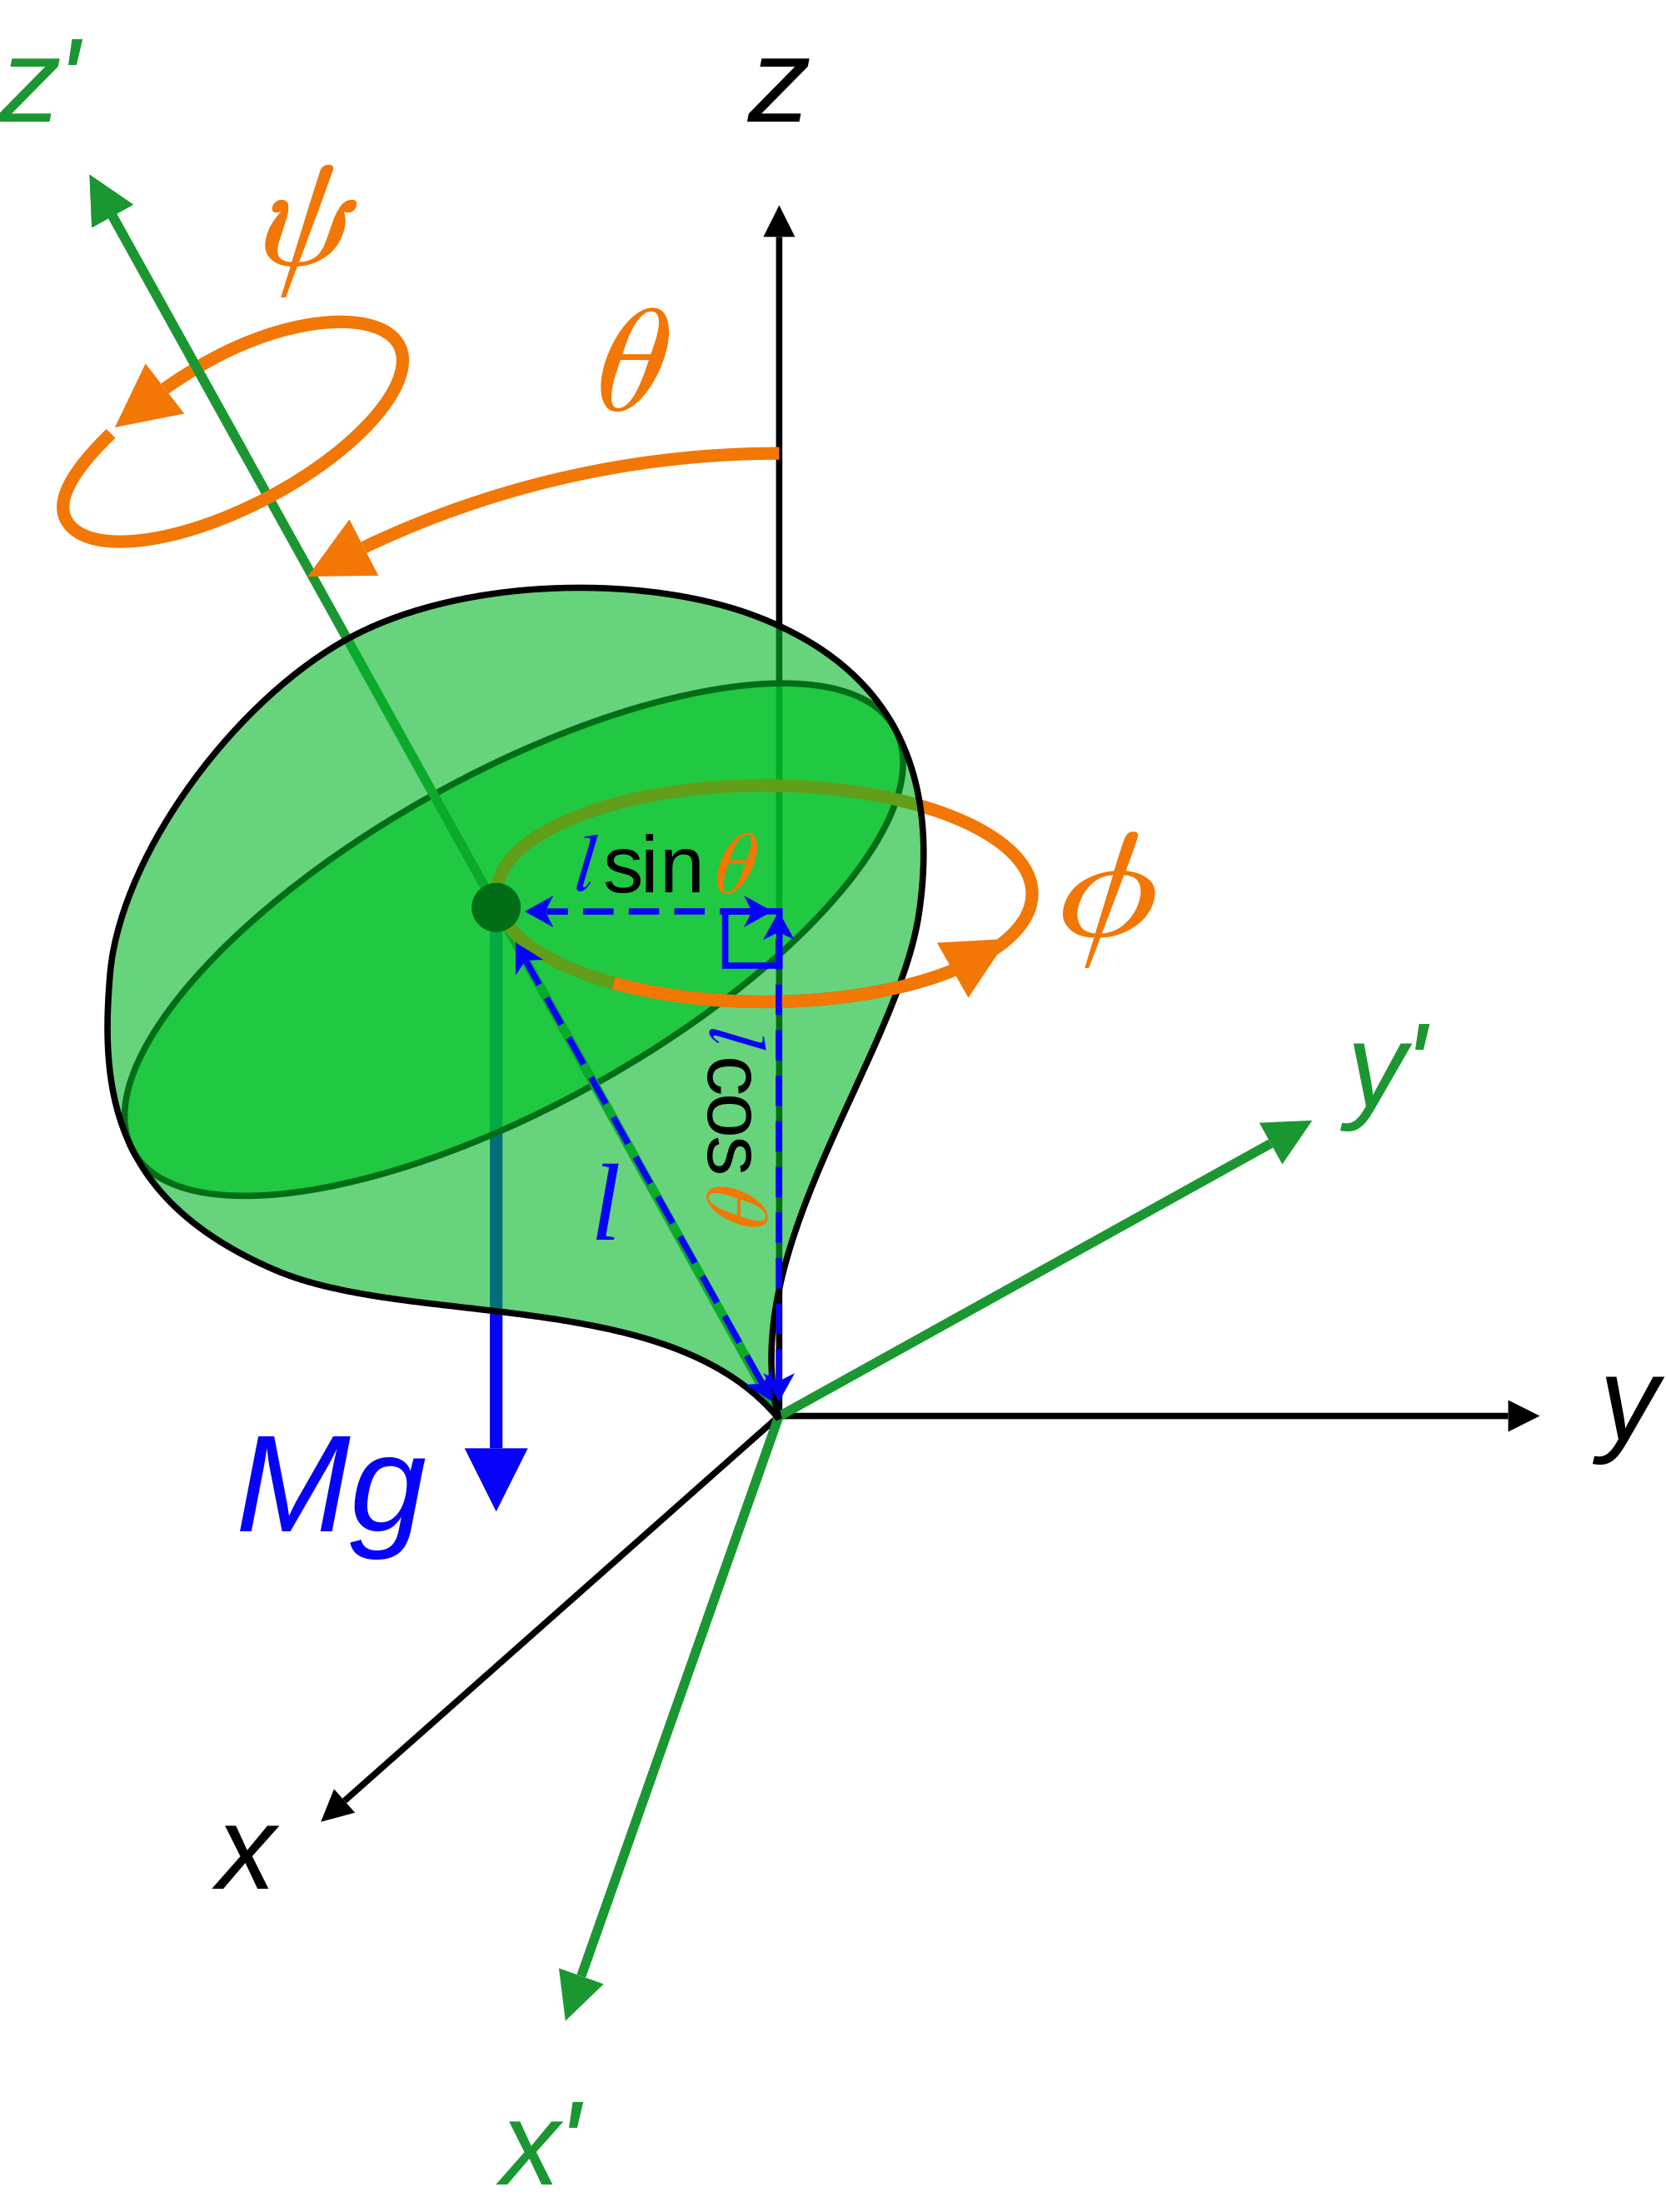
\includegraphics[width=\textwidth]{pics/eulertop}
    \caption{Trompo simétrico. Fuente: \cite{eulertop}.}
  \end{minipage}
  \end{figure}

  Inmediatamente tenemos
  \begin{align*}
    \dot{p_{\phi}} = & \parcial{H}{\phi} = 0 \\
    \dot{p_{\psi}} = & \parcial{H}{\psi} = 0,
  \end{align*}
  luego $p_{\phi}$ y $p_{\psi}$ son cantidades conservadas y por tanto su corchete de Poisson con $H$ se anula. Además, 
  \begin{equation*}
    \pois{p_{\phi}}{p_{\psi}} = 0.
  \end{equation*}
  Por tanto, $H$, $p_{\phi}$ y $p_{\psi}$ son funciones en involución en $(T^*\mathrm{SO}(3),H)$.

  Ahora, si estas funciones son constantes, como los ángulos (y sus relaciones trigonométricas) siempre están acotados también lo estará $p_{\theta}$ por la relación $E=H$ y la variedad $F^{-1}(a)$ estará acotada. Como $F^{-1}(a)$ es cerrada, es compacta y el trompo simétrico es «casi» un sistema integrable en el sentido de Liouville. Este «casi» viene porque, al igual que en el caso del péndulo habrá que exceptuar algún caso en el cual las funciones no son independientes.
\end{ejemplo}

\begin{ejemplo}
  \em
  Por citar un ejemplo no trivial, aunque no lo demostremos, el problema de hallar las geodésicas en un elipsoide puede verse como un sistema hamiltoniano integrable en el sentido de Liouville. La demostración se basa en la teoría de cuádricas confocales y coordenadas elípticas, demostrando unos teoremas de Jacobi y Chasles. Puede leerse en el apéndice 15 de \cite{arnold}.
\end{ejemplo}

Podemos probar ahora el resultado fundamental de esta teoría:
\begin{thm}[Arnold]
Sea $(M,H)$ un sistema integrable en el sentido de Liouville. Entonces:
\begin{enumerate}
  \item $M_a$ es una variedad diferenciable invariante bajo el flujo de hamiltoniano $H=F_1$ y $\omega|M_a=0$.
  \item Cada componente conexa $C_a$ de $M_a$ es difeomorfa al toro n-dimensional 
    \[
      \TT^n=\SF^1 \times \cdots \times \SF^1
    \]
    y, sean $\theta=(\theta_1,\dots,\theta_n)$ coordenadas angulares en $C_a$, entonces existen unas frecuencias constantes $\omega(a)=(\omega_1(a),\dots,\omega_n(a))$ tales que
    \[
    \dot{\theta}(t)=\omega.
    \]
    
\end{enumerate}

\end{thm}

\begin{proof}
  En primer lugar, como las $n$ funciones $F_i$ son independientes en cada punto de $M_a$, por el teorema de la función implícita $M_a$ es una subvariedad regular de $M$ de dimensión $2n-n=n$. 
  Como $M$ es una variedad simpléctica, para cada $i=1,\dots,n$, podemos definir el campo $X_i=X^{F_i}$. Al ser las $\dd F_i$ linealmente independientes los campos $X_i$ son linealmente independientes. Además, por el teorema de Noether, como para cada $i,j= 1,\dots,n$ $\pois{F_i}{F_j}=0$ (luego es constante), entonces $\lie{X_i}{X_j}=0$. Por esto mismo, la derivada de la función $F_i$ en la dirección de $X_j$ es 0, luego los campos $X_j$ son tangentes a $M_a$.

  De aquí sacamos varias conclusiones:
  \begin{enumerate}
    \item $M_a$ es invariante con respecto a cada uno de los $n$ flujos hamiltonianos generados por cada función $F_i$ (luego, en particular lo será respecto del generado por $F_1$).
    \item Como, para cada $x \in M_a$, los campos $X_1|_x,\dots, X_n|_x$ forman una base de $T_x M_a$, sean $X_x, Y_x \in T_x M_a$, entonces $X_x = \sum_{i=1}^n b_i X_i|_x$, $Y_x=\sum_{i=1}^n c_i X_i|_x$. Ahora,
      \[
	\omega(X_x,Y_x)= \sum_{i,j=1}^n b_i c_j \omega(X_i|_x,X_j|_x) = \sum_{i,j=1}^n b_i c_j \{F_j,F_i\} = 0.
      \]
      Por tanto, $\omega$ se anula en $T_x M_a$. 
    \item $M_a$ es una variedad diferenciable de dimensión $n$ con $n$ campos conmutativos dos a dos y linealmente independientes en todo punto de $M_a$. 
  \end{enumerate}

Por esto último, por la proposición anterior y porque $M_a$ es compacta tenemos que cada componente conexa $C_a$ de $M_a$ es difeomorfa a $\TT^n$. De la demostración de la proposición anterior obtenemos un diagrama de la forma:

\begin{center}
\begin{tikzpicture}
\node (A) at (-2.5,2) {$\RR^n$};
\node (B) at (-1,2) {$\RR^n$};
\node (C) at (-1,0) {$C_a=\TT^n$};
\node (D) at (1,2) {$\theta$};
\node (E) at (3,2) {$t$};
\node (F) at (3,0) {$\theta \mod 2\pi$};
\path[->,font=\scriptsize, >=angle 90]
(A) edge node[above]{$A$} (B)
(A) edge node[left]{$p$} (C)
(B) edge node[right]{$g$} (C);
\path[|->,font=\scriptsize, >=angle 90]
(D) edge node[auto] {$$} (F)
(D) edge node[auto] {$$} (E)
(E) edge node[auto] {$$} (F);
\end{tikzpicture}
\end{center}


En este caso, el flujo hamiltoniano asociado a $F_1$ es $g_1$, luego 
\[
\theta(t) = g_{1,t} (\theta(0)).
\]
Ahora, fijo $\theta(0)$, $g_{1,t}=g(t,0,\dots,0)$, por tanto
\[
\left(
\begin{array}{c}
\theta_1 (t)\\
\vdots \\
\theta_n (t)
\end{array}
\right)
=
A
\left(
\begin{array}{c}
t\\
0 \\
\vdots \\
0
\end{array}
\right).
\]
De modo que, si $a_{ij}$ es la entrada de índices $(i,j)$ de la matriz $A$, entonces, para cada $i=1,\dots,n$,
\[
\theta_i (t) = a_{i1} t.
\] 
Por tanto, sea $\omega_i=a_{i1}$,
\[
\dot{\theta_i}(t)=\omega_i.
\]
\end{proof}

\begin{obs}
  \em
  Estas subvariedades $C_a$ de $M$ se suelen llamar \textit{toros invariantes} del sistema $(M,H)$. 
  Esta dinámica en el toro recibe el nombre de \emph{movimiento condicionalmente periódico}.
\end{obs}

\begin{obs}
  \em
  Consideremos un 2-toro invariante con la dinámica del teorema (por ejemplo, el asociado a los niveles de energía de un oscilador armónico bidimensional). Sea $(\theta_1,\theta_2)$ un punto en el toro y su trayectoria bajo el flujo hamiltoniano $\gamma(t)=\varphi_t(\theta_1,\theta_2)=(\theta_1+\omega_1t,\theta_2+\omega_2t)$. Si $\omega_1/\omega_2=m/n$ es racional, entonces 
  \begin{equation*}
    \gamma\left(\frac{2n\pi}{\omega_2}\right) = (\theta_1+2m\pi,\theta_2+2n\pi)=(\theta_1,\theta_2).
  \end{equation*}
  Es decir, a cierto tiempo la trayectoria «se cierra». Estas órbitas se dicen \emph{periódicas}. 
 
  Sin embargo, si $\omega_2/\omega_1$ es irracional, dado un ángulo $\alpha$ y sea $T$ tal que $\alpha=\theta_1+\omega T$, entonces, sea $T_n=T+2n\pi/\omega_1$, $\alpha=\theta_1+\omega_1(T_n)$ para cada $n\in \NN$. Sea ahora la aplicación
  \begin{equation*}
    \begin{array}{rcl}
    g:\SF^1 & \longrightarrow &\SF^1 \\
  \phi & \longmapsto & \phi + 2\pi\frac{\omega_2}{\omega_1},
  \end{array}
\end{equation*}
es una rotación de ángulo un múltiplo irracional de $2\pi$ en la circunferencia del toro de ángulo $\alpha$. Entonces, como ya vimos por el teorema de recurrencia de Poincaré, $\{g^n(\phi)|n\in \NN\}$ es denso en $\SF^1$. Como esto es válido para todo $\alpha$ y se cumple 
\begin{equation*}
  \gamma(T_n)=(\alpha,g^n(\theta_2)+\omega_2 T),
\end{equation*}
tenemos que $\{\gamma(t)|t \in \RR \}$ es denso en el toro. Este tipo de órbitas se llaman \emph{cuasiperiódicas}. Una forma sencilla de visualizar esto es mediante las \emph{figuras de Lissajous} 
\begin{equation*}
  L_{\omega}=\{(\cos t, \cos \omega t) | t \in \RR\},
\end{equation*}
ver figura \ref{fig:lissajous}.
\begin{figure}[h]
  \centering
  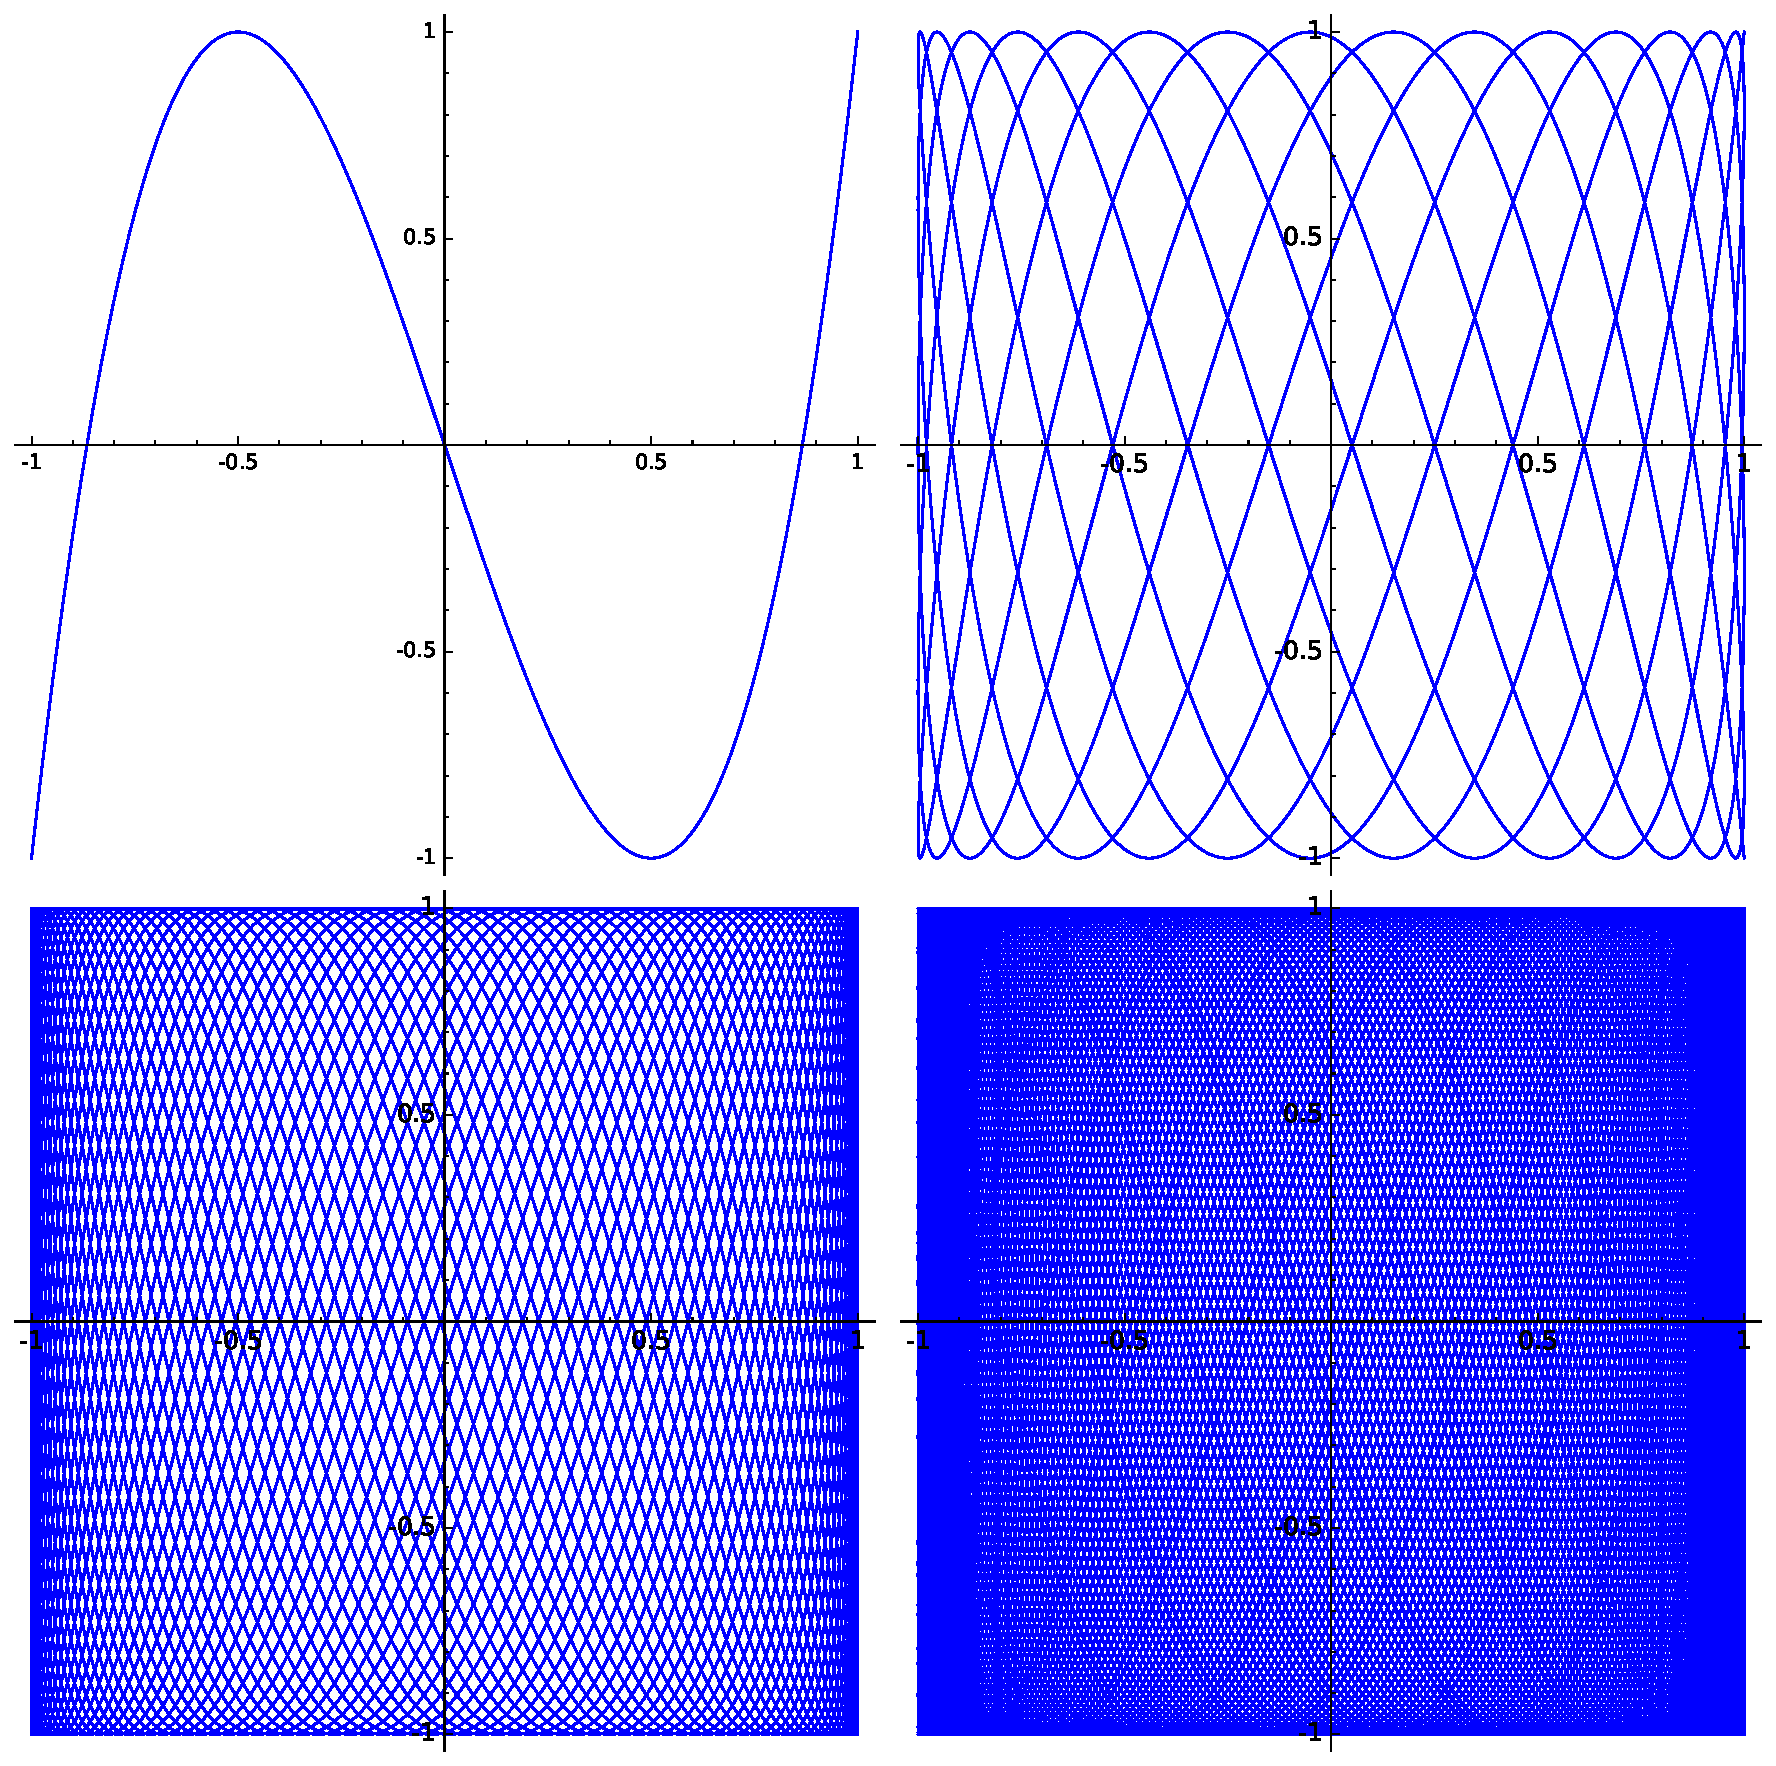
\includegraphics[width=0.6\textwidth]{pics/lissajous}
  \caption{Figuras de Lissajous para $\omega=3;3.1;3.14;3.1416$, $t \in (0,128\pi)$ con pasos de $0.01$.}
  \label{fig:lissajous}
\end{figure}
\end{obs}

Si $(M,H)$ es integrable en el sentido de Liouville, entonces para todo $x \in M$, $M_{F(x)}$ es compacta, luego la componente conexa a la que pertenezca $x$, $C_{F(x)}$, es un toro invariante, en el que podemos dar coordenadas angulares con una dinámica como la del teorema. A la vista de esto, tenemos el siguiente corolario:


Finalmente, vamos a demostrar el teorema clave que nos permite construir la carta en la cual las ecuaciones de Hamilton pueden ser integradas por cuadraturas.
\begin{thm}[de las variables de acción-ángulo]
  Sea $(M,H)$ un sistema integrable en el sentido de Liouville, $D \in \RR^n$ un disco, $a \in \RR^n$, $C_a$ un toro invariante y $U$ un entorno de $C_a$ difeomorfo a $\RR^n \times \TT^n$. Entonces existe un sistema de coordenadas simplécticas $(\phi,J)=(\phi_1,\dots,\phi_n,J_1,\dots,J_n)$ en $U$ tales que las $\phi_i$ son coordenadas angulares en cada toro invariante y las $J_i$ (comúnmente llamadas \emph{variables de acción}) son constantes en estos toros.
\end{thm}
\begin{proof}
  Sea $\pi:U\simeq \RR^n \times \TT^n \rightarrow \RR^n$ la proyección canónica, entonces $\pi^{-1}(x)$ es un toro invariante para cada $x \in D=\pi(U)$. En cada uno de estos toros, sean $X_i=X^{F_i}$ y $(F,\theta)$ las coordenadas obtenidas en el lema anterior,
\[
  \deriv{\theta_i} = \sum_{k=1}^n a_{ik}X_k,
\]
donde las $a_{ik}$ son funciones constantes en cada toro.

Como $\omega$ se anula en el toro, no tiene términos en $\dd \theta_i \wedge \dd \theta_j$. Los términos en $\dd \theta_i \wedge \dd F_j$ serán
\[
  \omega\left(\deriv{\theta_i},\deriv{F_j}\right)=\sum_{k=1}^n a_{ik}\cdot \omega\left(X_k,\deriv{F_j}\right)=\sum_{k=1}^n a_{ik} \cdot \dd F_k \left(\deriv{F_j}\right) = \sum_{k=1}^n a_{ik} \delta_{ij}= a_{ij}. 
\]
Por tanto, $\omega$ es de la forma
\[
  \omega = \sum_{i,j=1}^n a_{ij} \dd \theta_i \wedge \dd F_j + \sum_{i,j=1}^n b_{ij} \dd F_i \wedge \dd F_j,
\]
con $b_{ij}$ unas ciertas funciones. Además, como $\omega$ es cerrada, el término correspondiente a $\dd \theta_k \wedge \dd F_i \wedge \dd F_j$ debe anularse. Este término es exactamente
\[
  \parcial{a_{ki}}{F_j}-\parcial{a_{kj}}{F_i}+\parcial{b_{ij}}{\theta_k}.
\]
El término $\parcial{a_{ki}}{F_j}-\parcial{a_{kj}}{F_i}$ no depende de las variables angulares, luego las $\parcial{b_{ij}}{\theta_k}$ son constantes al variar los ángulos $\theta_k$. Como las variables $\theta_k$ son angulares, las $b_{ij}$ deben ser periódicas, luego
\[
  \parcial{b_{ij}}{\theta_k}=0
\]
y las $b_{ij}$ son constantes en cada toro invariante.

Si ahora definimos $A_i=\sum_{j=1}^n a_{ij}\dd F_j$, $B=\sum_{i,j=1}^n b_{ij}\dd F_i \wedge \dd F_j$,
\[
  \omega=\sum_{i=1}^n \dd \theta_i \wedge A_i + B.
\]
Como las $a_{ij}$ y las $b_{ij}$ son constantes en cada toro invariante podemos ver las $A_i$ y $B$ como formas en $\RR^n$, es decir, existen 1-formas $\alpha_i$ y una 2-forma $\beta$ en $\RR^n$ tales que
\[
  A_i= \pi^* \alpha_i \hspace{1cm} B=\pi^* \beta.
\]
De aquí tenemos
\[
  0=\dd \omega= \sum_{i=1}^n \dd \theta_i \wedge \pi^* \dd \alpha_i + \pi^* \dd \beta,
\]
de donde concluimos que $\dd \alpha_i = 0$ y $\dd \beta =0$. En $\RR^n$ todas las formas cerradas son exactas. Por tanto, existen $I_i$ y $\gamma$ en $\RR^n$ tales que $\alpha_i = \dd I_i$, $\beta= \dd \gamma$.

Finalmente, sean $J_i=(I_i \circ \pi)=\pi^* I_i$, tenemos que $\dd J_i = A_i$, luego
\[
  \omega = \sum_{i=1}^n \dd \theta_i \wedge \dd J_i + B.
\]
En el sistema de coordenadas $(\theta,F)$, la matriz asociada a $\omega$ es de la forma
\[
\left(
\begin{array}{c|c}
  0 & \parcial{J_i}{F_j} \\
  \hline 
  -\parcial{J_i}{F_j} & b_{ij}
\end{array}\right).
\]
Como $\omega$ es regular, el determinante de esta matriz es distinto de cero, luego $\det\left(\parcial{J_i}{F_j}\right)\neq 0$. Por tanto, $(\theta,J)$ es un sistema de coordenadas.

Ahora, si escribimos $\gamma= \sum_{i=1}^n g_i \dd I_i$, para algunas funciones $g_i:\RR^n \rightarrow \RR$, entonces podemos tomar unas nuevas coordenadas 
\[
  \phi_i= \theta_i + (g_i \circ \pi).
\]
En estas nuevas coordenadas
\[
\begin{split}
  \sum_{i=1}^n \dd \phi_i \wedge \dd J_i & = \sum_{i=1}^n \dd \theta_i \wedge \dd J_i + \sum_{i=1}^n \dd(g_i \circ \pi) \wedge J_i \\
   & =\sum_{i=1}^n \dd \theta_i \wedge \dd J_i + \sum_{i=1}^n \dd(g_i \circ \pi) \wedge \dd (I_i \circ \pi) \\
   & =\sum_{i=1}^n \dd \theta_i \wedge \dd J_i + \pi^* \dd \gamma = \sum_{i=1}^n \dd \theta_i \wedge A_i + B = \omega.
\end{split}
\]

Por tanto, hemos encontrado unas coordenadas simplécticas $(J,\phi)$, con las $J_i$ constantes en cada toro invariante y con las $\phi_i$ coordenadas angulares en estos toros.
\end{proof}

\begin{obs}
  \em
  Volviendo al caso del oscilador armónico $n$-dimensional, notamos que $\omega=\dd \alpha$, con $\alpha=\sum_{i=1}^n J_i \dd \phi_i$, entonces $J_i=\frac{1}{2\pi}\int_{\gamma_i}\alpha$.
\end{obs}

\begin{corol}
  Todo sistema integrable en el sentido de Liouville es integrable por cuadraturas.
\end{corol}

\begin{proof}
  Dado un punto $x \in M$, basta tomar unas variables de acción-ángulo (las $(J,\phi)$ del teorema). Entonces, como ya hemos visto, las soluciones de las ecuaciones de Hamilton en estas coordenadas quedan escritas en la forma
  \begin{align*}
    J_i(t) & = J_i (0) \\
    \phi_i(t) & = \phi_i(0) + \omega_i(F(0))t,
  \end{align*}
  para $i=1,\dots,n$, donde las frecuencias $\omega_i$ se obtuvieron en términos de funciones conocidas. Así, el sistema queda integrado por cuadraturas.
\end{proof}



